%%  ***************************************************************************
%% My paper
%%
%% Authors: Emmett Brown, Marty McFly, Biff Tannen
%%
%% NOTE: this file will not compile until you called the script
%% generate-preamble.php once. See the file Readme.md to understand what
%% to do.
%%
%% This paper is an instance of the PaperShell template. For more
%% information, please visit https://github.com/sylvainhalle/PaperShell
%%  ***************************************************************************
%% ---------------------------
%% Author preamble. Uncomment the one corresponding to the
%% stylesheet you want. **Don't forget to also uncomment the proper
%% line for the postamble at the end!!**
%% ---------------------------
%\input preamble-aaai.inc.tex
%\input preamble-acm.inc.tex
%\input preamble-acm-journal.inc.tex
%\input preamble-elsarticle.inc.tex
%\input preamble-ieee.inc.tex
%\input preamble-ieee-journal.inc.tex
\input preamble-lncs.inc.tex
%\input preamble-svjour.inc.tex

%% ---------------------------
%% If you wish to include additional packages, define new environments or
%% new commands, put them in the file includes.tex
%%
%% Write your abstract in the file abstract.tex.
%% ---------------------------

%% ---------------------------
%% Categories and keywords. Uncomment only for ACM.
%% See: http://www.acm.org/about/class/ccs98-html
%% ---------------------------
\begin{comment}
  \category{D.2.2}{Software Engineering}{Design Tools and Techniques}
  \category{D.2.4}{Software Engineering}{Software/Program Verification}
  \category{H.3.5}{In\-for\-ma\-tion Storage and Retrieval}{Online Information Services}[web-based services]
  \terms{Theory, verification}
  \keywords{Navigation, web applications, model checking}
  \vfill\eject
\end{comment}

%% ---------------------------
%% Introduction
%% ---------------------------
\section{Introduction} %% {{{

Fault localization. 

While lot of work has been done on reporting the presence of an error, much less has been done on localizing the fault, i.e.\ identifying artifacts providing a meaningful explanation for the occurrence of the fault.

%% }}} --- Section


%% ---------------------------
%% Witnesses
%% ---------------------------
\section{Applications} %% {{{

\subsection{Configuration Management}

Narain

\subsection{Web Applications}

%% }}} --- Section

%% ---------------------------
%% Witnesses
%% ---------------------------
\section{Defining Witnesses} %% {{{

Let $\mathcal{D}$ be a set of \emph{domain elements}, with a special element $\sz \in \mathcal{D}$ we shall name the \emph{empty} element. Let $\Tau$ be a set of transformations; each transformation $\tau$ is an endomorphism over $\mathcal{D}$, i.e.\ a function $\tau : \mathcal{D} \rightarrow \mathcal{D}$.

Transformations can be composed in the usual way, i.e.\ $\tau \circ \tau'$ is the endomorphism $\tau''$ such that $\tau''(d) = \tau(\tau'(d))$ for every $d \in \mathcal{D}$. We further expect this composition to be associative and commutative. Then, given a set of transformations $T \subseteq \Tau$, we will note as $\bigcirc T$ the composition of every transformation in $T$; that is, if $T = \{\tau_1, \dots, \tau_n\}$, then $\bigcirc T = \tau_1 \circ \dots \circ \tau_n$. Since we suppose that composition is commutative, the resulting transformation is well defined. Set inclusion induces a partial ordering over sets of transformations.


Let $\Phi$ be a set of \emph{language expressions} equipped with a satisfaction relation $\models : \mathcal{D} \times \Phi \rightarrow \{\top,\bot,?\}$. For an expression $\varphi \in \Phi$ and a domain structure $d \in \mathcal{D}$, we will abuse notation and write $d \models \varphi$ if and only if $\models(d,\varphi) = \top$.

Let $d \in \mathcal{D}$ be a structure such that $d \not\models \varphi$ for some expression $\varphi \in \Phi$. A \emph{witness} is defined as a set of transformations $T \subseteq \Tau$ such that:
%
\begin{enumerate}
\item $\bigcirc T(d) \models \varphi$
\item For every $T' \in \Tau$, either $\bigcirc T'(d) \not\models \varphi$ or $T \subseteq T'$.
\end{enumerate}

Intuitively, a witness is a set of ``changes'' to a domain element $d$ that make it satisfy $\varphi$, such that no ``smaller'' change restores satisfiability. Since $\subseteq$ is a partial order, there may be multiple, mutually uncomparable witnesses.

\subsection{Propositional Logic}

As a first example, let $\Phi$ be the set of propositional logic formul\ae{} with at most $n$ variables $x_1, \dots, x_n$ for some $n \geq 1$. Let $\mathcal{D}$ be the set of functions $\{\top,\bot\}^n \rightarrow \{\top,\bot\}$, which we shall call \emph{valuations}. The satisfaction relation $\models$ is defined as $\models(d, \varphi) = \top$ if $\varphi$ evaluates to true when its variables are replaced by the corresponding truth value specified by $d$, and $\bot$ otherwise.

Let $b \in \{\top,\bot\}$ and $i \in [1,n]$. We will note $\tau_{x_i,b}$ to denote the transformation $\tau_{x_i,b} : d \mapsto d[x_i/b]$. This transformation sets $x_i$ to $b$ and leaves the rest of the input valuation unchanged. The set of transformations $\Tau$ is then defined as:
\[
\Tau \triangleq \{\tau_{b,x_i} : i \in [1,n]\mbox{ and }b \in \{\top,\bot\}\}
\]

\begin{example}
Let $d$ be the valuation $\{a \mapsto \top, b \mapsto \bot, c \mapsto \bot\}$ and $\varphi$ the propositional formula $a \wedge b$. One can easily observe that $d \not\models \varphi$. A witness is the set of transformations $T= \{\tau_{b,\top}\}$. This corresponds to the intuition that the explanation for the falsehood of $\varphi$ is that $b$ is false while it should be true. Note that although $T'=\{\tau_{b,\top}, \tau_{c,\top}\}$ would also make $\varphi$ true, it does not count as a witness, since $T \subseteq T'$. This corresponds to the intuition that the truth value of $c$ is not relevant to the falsehood of $\varphi$.
\end{example}

\begin{example}
Let $d$ be the valuation $\{a \mapsto \top,b \mapsto \bot,c \mapsto\bot\}$ and $\varphi$ the propositional formula $a \rightarrow b$. This time, two witnesses exist: $T= \{\tau_{b,\top}\}$ and $T' = \{\tau_{a,\bot}\}$. It is possible to check that both fix the truth value of the original valuation. Informally, the first witness accounts the falsehood of $\varphi$ on the fact that $a$ is true, while the other one rather explains it by the fact that $b$ is false ---which indeed corresponds to the intuition. Since both witnesses are uncomparable, none of these explanations is ``preferred''.
\end{example}

\todosylvain{Faire un lien entre ceci et le incremental SAT}


\subsection{First-Order Logic}

The concept of witness can easily be lifted to the set $\Phi$ of first-order logic formul\ae{} on finite domains. Let $A$ be a set of elements; an $n$-ary predicate is defined as a function $p : A^n \rightarrow \{\top,\bot\}$; let $P^i$ be the set of predicates of arity $i$. A signature is a set of predicates $\{p_1, \dots, p_m\}$, respectively of arity $a_1, \dots, a_m$. For a given signature, the set of domain elements is defined as:
\[
\mathcal{D} \triangleq P^{a_1} \times \dots \times P^{a_m}
\]

The satisfaction relation $\models$ is defined as $\models(d, \varphi) = \top$ if $\varphi$ evaluates to true when evaluating predicates as defined in $d$, and $\bot$ otherwise.

In this context, a transformation will represent the change in the truth value for one input of one predicate. Let $p_k$ be a predicate of arity $i$, $(a_1, \dots, a_k) \in A^n$ be a $k$-tuple of elements of $A$, and $b \in \{\top,\bot\}$. The transformation $\tau_{p_k,(a_1,\dots,a_k),b}$ is defined as the predicate $p_k'$ such that:
\[
p_k'(x_1,\dots,x_k) = 
\begin{cases}
b & \mbox{if $x_1 = a_1$, \dots, $x_n = a_n$}\\
p_k(x_1,\dots,x_k) & \mbox{otherwise}
\end{cases}
\]

The set of transformations for $p_k$, noted $T_{p_k}$, is defined as:
\[
T_{p_k} \triangleq \bigcup_{(a_1,\dots,a_k)\in A^n} \left(\bigcup_{b \in \{\top,\bot\}} \{\tau_{p_k,(a_1,\dots,a_k),b}\}\right)
\]

The global set of transformations is then:
\[
\mathcal{T} \triangleq \bigcup_{i \in [1,m]} T_{p_i}
\]

\begin{example}
Let $A = \{0,1,2\}$, $\varphi$ be the first-order formula $\forall x : \exists y : p(x,y)$, and the binary predicate $p$ defined as $\{(0,0), (0,1), (1,1)\}$. There are three witnesses for restoring the truth of $\varphi$: $T_1=\{\tau_{p,(2,0),\top}\}$, $T_2=\{\tau_{p,(2,1),\top}\}$, $T_3=\{\tau_{p,(2,2),\top}\}$.m
\end{example}

\begin{example}
Let $A = [1,5]$ be a set of graph vertices, $p$ a binary predicate encoding the adjacency relationship ofn graph edges, and $q_1$,$q_2$,$q_3$ a set of unary predicates such that $q_i(x)$ holds if and only if vertex $x$ has color $i$. Predicates $p$ and $q$ are defined according to the graphical representation shown in Figure \ref{fig:graph-original}.

\begin{figure}
\begin{center}
\subfloat[Original graph]{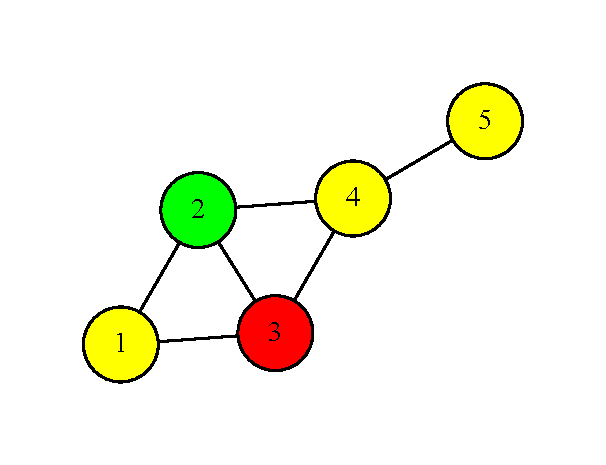
\includegraphics[width=1.5in]{fig/graph-coloring-1}\label{fig:graph-original}}
%
\subfloat[After applying $T_1$]{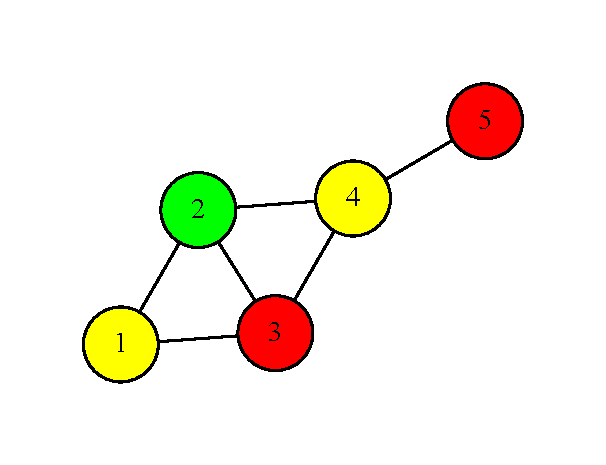
\includegraphics[width=1.5in]{fig/graph-coloring-t1}\label{fig:graph-t1}}
%
\subfloat[After applying $T_3$]{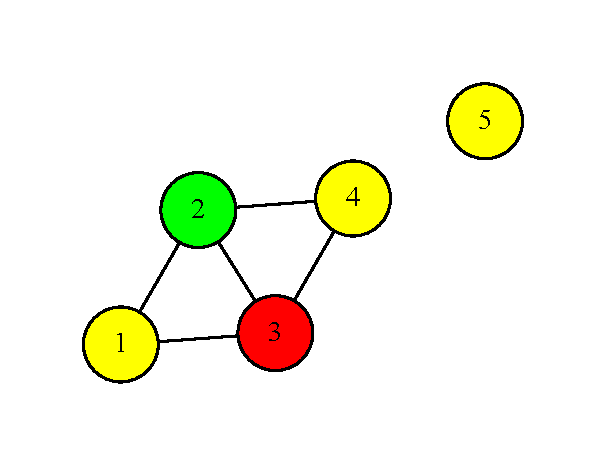
\includegraphics[width=1.5in]{fig/graph-coloring-t3}\label{fig:graph-t3}}
\\
%
\subfloat[After applying $T_4$]{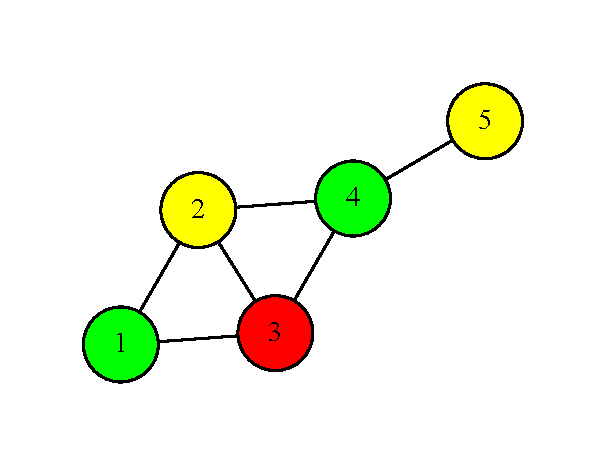
\includegraphics[width=1.5in]{fig/graph-coloring-t4}\label{fig:graph-t4}}
%
\subfloat[After applying $T_5$]{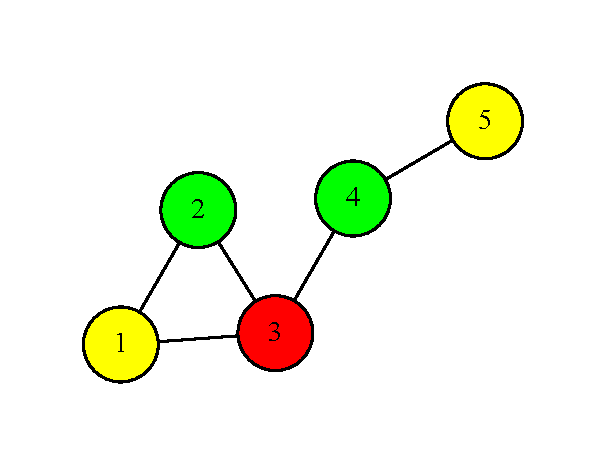
\includegraphics[width=1.5in]{fig/graph-coloring-t5}\label{fig:graph-t5}}
\caption{Encoding of a graph}
\end{center}
\end{figure}

Let $\varphi_1$ be the following first-order formula:
\begin{multline*}
\varphi_1 \triangleq \forall x : (q_1(x) \rightarrow \neg(q_2(x) \vee q_3(x))) \wedge (q_2(x) \rightarrow \neg(q_1(x) \vee q_3(x))) \wedge \\
(q_3(x) \rightarrow \neg(q_1(x) \vee q_2(x)))
\end{multline*}
%
\begin{displaymath}
\varphi_2  \triangleq  \forall x : q_1(x) \vee q_2(x) \vee q_3(x)
\end{displaymath}
%
\begin{multline*}
\varphi_3  \triangleq  \forall x : \forall y : p(x,y) \rightarrow\\
((q_1(x) \rightarrow \neg q_1(y)) \wedge (q_2(x) \rightarrow \neg q_2(y)) \wedge (q_3(x) \rightarrow \neg q_3(y)))
\end{multline*}
%
\begin{displaymath}
\varphi_4  \triangleq  \forall x : \forall y : p(x,y) \rightarrow p(y,x)
\end{displaymath}
%
Intuitively, $\varphi_1$ stipulates that each vertex can be of at most one colour, $\varphi_2$ imposes that each vertex be of at least one colour, and $\varphi_3$ expresses the fact that two adjacent vertices cannot be of the same colour. Finally, $\varphi_4$ ensures that the connectivity is symmetric.

One can see that the original graph does not satisfy $\varphi_1 \wedge \varphi_2 \wedge \varphi_3$. There are multiple witnesses, a few of which are shown here:
\[
T_1 = \{\tau_{q_1,5,\bot},\tau_{q_2,5,\top}\}
\]
\[
T_2 = \{\tau_{q_1,5,\bot},\tau_{q_3,5,\top}\}
\]
\[
T_3 = \{\tau_{p,(4,5),\bot},\tau_{p,(5,4),\bot}\}
\]
\[
T_4 = \{\tau_{q_1,1,\bot},\tau_{q_3,1,\top},\tau_{q_1,4,\bot},\tau_{q_3,4,\top}\}
\]
\[
T_5 = \{\tau_{p,(2,4),\bot},\tau_{p,(4,2),\bot},\tau_{q_1,4,\bot},\tau_{q_3,4,\top}\}
\]
% Yellow = 1
% Red = 2
% Green = 3

Witness $T_1$ fixes the graph by changing the colour of vertex 5 to red; similarly, $T_2$ changes it to green. Witness $T_3$ rather alters the adjacency relation and cuts vertex 5 from the graph, so that the colour conflict is resolved.

These correspond to the ``intuitive'' ways of fixing the graph colouring. However, there exist multiple other witnesses that fulfill the definition. For example, witness $T_4$ rather exchanges the colours of vertices 1, 2 and 4. Note that this is indeed a witness, in that no subset of these transformations restore satisfiability of the original formula.

In the same way, $T_5$ cuts the edge between vertices 2 and 4, and turns 4 to green.
\end{example}

Again, it should be noted that without additional context, none of these witnesses is a more likely explanation to the falsehood of $\varphi_1 \wedge \varphi_2 \wedge \varphi_3$ on the original graph.

\todosylvain{Ménage dans les noms symboles}

\subsection{Temporal Logic}

Let $\Sigma$ be an alphabet of atomic symbols, and $\Sigma^*$ the set of finite traces made from symbols of $\Sigma$.

Define the ordering relation 

%% }}} --- Section


%% ---------------------------
%% Witnesses
%% ---------------------------
\section{Computing Witnesses} %% {{{



%% }}} --- Section

%% ---------------------------
%% A section
%% ---------------------------
\section{Conclusion} %% {{{

It works.


%% }}} --- Section

%% ---------------------------
%% Bibliography. Uncomment the one corresponding to the
%% stylesheet you want.
%% ---------------------------
%\input postamble-aaai.inc.tex
%\input postamble-acm.inc.tex
%\input postamble-acm-journal.inc.tex
%\input postamble-elsarticle.inc.tex
%\input postamble-ieee.inc.tex
%\input postamble-ieee-journal.inc.tex
\input postamble-lncs.inc.tex
%\input postamble-svjour.inc.tex

\end{document}

%% :folding=explicit:wrap=soft:mode=latex:
